% next time: measure sides of object, report in sig figs, and calculate diagonal


\documentclass[11pt,letterpaper]{article}
\usepackage{array}
\usepackage{fullpage}
\usepackage{graphicx}
\usepackage{parskip}
\usepackage{amsmath}
\usepackage[small]{caption}
\usepackage{graphpap}
\usepackage{tabularx}
\usepackage{url}
\usepackage{hyperref}
\usepackage{enumitem}

\renewcommand{\thesection}{PART \arabic{section}: }

\newcounter{question}[section]
\newenvironment{question}[1][]{\refstepcounter{question}\par\medskip
   \textbf{\arabic{section}.\thequestion.} \rmfamily}{\medskip}

\usepackage{titlesec}
\titleformat{\section}{\clearpage\normalfont\bfseries}{\thesection}{0em}{}
\titlespacing{\section}{0pt}{0.5\baselineskip}{0pt}

\titleformat{\subsection}[runin]
{\normalfont\bfseries}{\thesubsection}{1em}{}

\titleformat{\subsubsection}{\normalfont\bfseries}{\thesubsubsection}{0em}{}
\titlespacing{\subsubsection}{0pt}{0.5\baselineskip}{0pt}

\newcounter{saveenumi}
\newcommand{\seti}{\setcounter{saveenumi}{\value{enumi}}}
\newcommand{\conti}{\setcounter{enumi}{\value{saveenumi}}}

\usepackage[dvipsnames]{xcolor}
\newcommand{\sol}[1]{{\color{NavyBlue} #1}}

\begin{document}
\setlength{\parindent}{0in}
%next time fix vernieer calipers problem by adding units.
%2.1 label parts of graph
%% EQUIPMENT: ruler, caliper, micrometer, logger, motion sensor

\begin{flushright}
Physics S123\\
Lab 1: Measurements and Motion\\
8/24/21 (due 8/31/21)
\end{flushright}

Name(s):\\


\subsubsection*{Topics:}
\begin{enumerate}
\setlength{\parskip}{3pt}
\item Measurement with rulers and calipers; precision and significant figures
\item Measurement uncertainty
\item Computer data acquisition software and equipment
\item Graphical analysis of data
\end{enumerate}

\subsubsection*{Introduction:}
The lab consists of four parts that are designed to give you familiarity with the above topics. Subsequent labs and homework assignments will build on these basic ideas and methods. Throughout the semester you will collect motion data with LoggerPro. To assist with data analysis and graphing, you will also learn some basic MATLAB programming. MATLAB is a high-level program that is relatively easy to learn, has very good help files, and can be used either as a calculator or as a programming language. 

LoggerPro and MATLAB are both installed on the university build, which you can access from your computer. Instructions for accessing the university's virtual machine can be found here: \url{https://uas.alaska.edu/helpdesk/computers/central/virtual.html}. Note that you will also need to use VPN if you are attempting to access the virtual machine from off campus.
Keep in mind that when using the virtual machine you should save files to your Z drive (or google drive or email them to yourself). If you save them elsewhere on the machine the files will disappear when you log out.

\subsubsection*{What you should turn in:}
An informal lab report. You may submit a group report if you'd like. Answer the questions and submit graphs where indicated. You can submit your answers on this handout or typed in a separate document. In particular, I am looking for: 
\begin{itemize}
\setlength{\parskip}{3pt}
\item Section 1: Measurements and instrument uncertainties [2 pts]
\item Section 2.1: Which errors are systematic and/or random, and why? [2 pts]
\item Section 2.2: Calculation of uncertainty using the crank three times method [2 pts]
\item Section 2.3: Calculation of uncertainty using standard deviations [2 pts]
\item Section 3.1: Motion graphs, plotted using MATLAB [4 pts]
\item Section 3.2--3.4: Screen shots of the matching exercises and a description of the graphs [2 pts]
\item Section 3.5: Screenshots of your measurements [2 pts]
\item Section 4.1: Graphs (linear, semilogx, semilogy, or log-log) of the data that most closely resemble straight lines [2 pts]
\item Section 4.2: Calculation of the power-law relationship between orbital period and radius [2 pts]
\end{itemize}

\subsubsection*{Equipment:}
\begin{itemize}
\setlength{\parskip}{3pt}
\item Ruler
\item Vernier calipers
\item LabQuest interface, cables, and motion sensor
\end{itemize}

\section{MEASUREMENT AND RESOLUTION}
When making measurements it's always important to understand the limitations of the instruments that you are using. In part 1 you will gain a better understanding of instrument resolution by making measurements with a ruler and with a calipers. These instruments have different levels of resolution:
\begin{table}[h]
\begin{tabular}{ll}
Instrument \hspace*{5mm} & resolution\\
\hline
Ruler & 1 mm\\
Calipers & 0.05 mm\\
%Micrometer & 0.01 mm\\
\hline
\end{tabular}
\end{table}\\
Resolution refers to the smallest increment of an instrument; the uncertainty of an \textit{individual} measurement is found by diving the resolution by 2. In other words,
$$\mbox{uncertainty}=\pm\frac{\mbox{resolution}}{2}.$$

The number of digits that you record during a measurement should reflect the number of digits that you have confidently measured. This is referred to as significant figures. Rules for recording measurements and applying arithmetic operations to those numbers:
\begin{itemize}
\item When recording a measurement, write down all of the digits that are known precisely plus one digit that is estimated. For example, you might use a ruler to measure the width of a piece of paper as 21.59$\pm$0.05 cm. The last digit (9) is uncertain because the ruler only has markings every 0.1 cm.
\item Only record zeros if they are located between non-zero digits or trail a number if they come after the decimal place.
\item Zeros can be ambiguous. How many significant figures does 21,000 have? For this reason it's often better to use scientific notation. $2.1000\times{10^4}$ has five significant figures, while $2.10\times{10^4}$ has only three.
\item When adding or subtracting, the answer should have the smallest number of decimal places of the numbers used in the calculation.
\item When multiplying or dividing, the answer should have as many significant figures as the number used in the calculation that has the smallest amount of significant figures.
\item Only apply significant figures to measured values (not countables, $\pi$, or other known constants). 
\item \textbf{Don't round during intermediate calculations!}
\end{itemize}
If you follow these rules correctly, the last digit will be the only uncertain digit. The reason that significant figures is important is that they give the reader an idea of the measurement precision.

\clearpage
\question{} Make measurements using a ruler. Select a convenient object (note what object you are using) and make three or more measurements. Report the length and uncertainty of each measurement. Be sure to include the correct number of significant figures in your measurements.
\vspace{6cm}


\question{} Repeat Experiment 1 using the vernier calipers to measure some dimension of an object (again, note which object). Repeat the \textit{same} measurement 10 times (yes, this is tedious, but you will use this data in Section 2.3 to estimate error).



\section{UNCERTAINTY}
Consider an observable $x$. It could be a length, a mass, a volume, etc. A random error in the measurement of $x$
is an error that changes from measurement to measurement, while a
systematic error is one that persists with each measurement.  A bit
more precisely:  a systematic error is one that is due to the
measuring equipment (or process) itself, and is therefore
reproducible.  A random error is an error that is
statistical in nature and therefore in principle irreproducible.
Examples of random errors include the way we hold a meter stick or the
angle of our eye while reading it.  An example of a systematic error
arises when a poorly printed ruler has the length of each centimeter
equivalent to 11 millimeters.

Systematic errors can be determined and eliminated by changing measurement methods.  Random errors are those whose causes are unknown and cannot be eliminated.  Since random errors occur by chance, their effect on experimental results may be minimized by taking as many observations as possible.

\question{} All measurements can lead to random errors. Which of the following also lead to systematic errors, and why?\\
a. The end of a ruler was used in measuring lengths.\\
b. The duration of an event is measured by starting and stopping a stopwatch.\\
c. A volume is determined by measuring the displacement of water in a
graduated cylinder.\\
d. The weight of an object is measured on a bathroom scale that reads 2 pounds when unused.\\
\vspace{6cm}

\question{} Significance vs. uncertainty

Significant figures are not a good indication of uncertainty. They simply tell you how many digits to report in a measurement or calculation involving measurements. Consider the resolution of the ruler and of the calipers. The ruler has a resolution of 1 mm. A ruler measurement should be reported as 21.69 cm, where the last digit is uncertain. The uncertainty in the measurement is half the resolution, or $\pm$0.05 cm. This tells you that the actual value is between 21.64 cm and 21.74 cm. The calipers on the other hand, has a resolution of 0.05 mm. A calipers measurement should be reported as 1.384 cm, where the last digit is uncertain. The uncertainty is $\pm$0.025 mm ($\pm$0.0025 cm), so that the actual value is between 1.3815 cm and 1.3865 cm. In this case, the number of significant figures in the reported value doesn't tell you the uncertainty (it overestimates it). 

Furthermore, even if the number of significant figures did tell you the uncertainty of a measurement, it's not always clear how to propagate that uncertainty through a calculation. A simple way to estimate the uncertainty of a calculation is to use the ``crank three times'' method. Here's how it works:
\begin{enumerate}
\item Make your calculation using the estimated value of your measurements.
\item Repeat, this time using the minimum bound of your measurements.
\item Repeat, this time using the maximum bound of your measurements.
\end{enumerate}
When reporting your result, it's good to show the mean and the minimum and maximum bounds. In all cases, use the rules of significant figures to determine how many digits to present.

Let's try it out by finding the hypotenuse of a right triangle. One leg of the triangle is 13.3632 cm $\pm$0.00025 cm, and the other leg is 5.2 cm $\pm$0.5 cm. What are the mean and maximum and minimum possible values of the hypotenuse? HINT: All three results should have three significant figures, and the first two numbers should agree -- remember, the last digit is the only uncertain digit!
\vspace{10cm}



\question{} When measurements have random errors, the measured values will have a normal (or bell-shaped) distribution around the mean. Normal distributions are well understood mathematically. When numerous measurements are made, we can obtain an improved estimate of the measurement uncertainty by calculating the standard deviation, $s$,
\begin{equation*}
s=\sqrt{\frac{\displaystyle\sum_{i=1}^N(x_i-\overline{x})^2 }{N-1}},
\end{equation*}
where $x_i$ indicate the individual measurements, $\overline{x}$ is the average of the measurements, and $N$ is the total number of measurements. For random measurement errors, 68.2\% of all measurements are within one standard deviation of the population mean; 95.6\% of all measurements are within two standard deviations.
\begin{figure}[h!]
\begin{center}
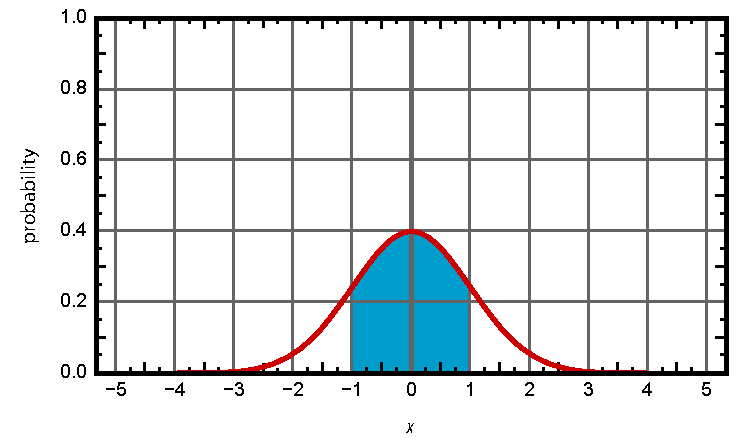
\includegraphics[]{./bell_curve}
\end{center}
\caption*{Example of a bell-shaped curve. In this example, the mean is $\overline{x}=0$ and the standard deviation is $s=1$. There is a 68.2\% probability that all measurements will fall within the shaded region (between $x=-1$ and $x=1$). The values of the mean and standard deviation depend on your data set.}
\end{figure}

Calculate the mean and standard deviation of your caliper measurements (problem 1.2). Is the standard deviation larger or small than the uncertainty associated with individual measurements?

Use MATLAB to calculate the standard deviations using the following commands (in the command window). You do not need to submit anything for each of these steps; this is just to give you some feel for making calculations with MATLAB.

 
Create a vector containing your data:
\begin{verbatim}>> data=[number, number, number, ...];\end{verbatim}
Note that the semicolon suppresses output to the screen. Try typing it again
without the semi-colon to see what happens.

Add all of the data points.
\begin{verbatim}>> sum(data)\end{verbatim}

Find the number of elements in the data vector.
\begin{verbatim}>> length(data)\end{verbatim} 

Calculate the mean.
\begin{verbatim}>> sum(data)/length(data)\end{verbatim}

Now calculate the mean using MATLAB's built-in function.
\begin{verbatim}>> mean(data)\end{verbatim}

Subtract the mean from each data point.
\begin{verbatim}>> data-mean(data)\end{verbatim}

Remove the mean and square each term. 
\begin{verbatim}>> (data-mean(data)).^2\end{verbatim}
The \verb!.^! is for element-by-element multiplication. If you don't include the period, MATLAB will try to use matrix multiplication.

Calculate the standard deviation.
\begin{verbatim}>> sqrt(sum((data-mean(data)).^2)/(length(data)-1))\end{verbatim}
Report your result here:

\bigskip
\bigskip
MATLAB, like other programs, has a built-in command for calculating the standard deviation. Try the following:
\begin{verbatim}>> std(data)
\end{verbatim}
Report your result here:

\section{VISUALIZING MOTION WITH GRAPHS}
In this section you will become familiar with the Logger Pro data acquisition software and equipment that we will use throughout the semester.

After completing these exercises, you should be able to look at distance-time and velocity-time graphs and describe the motion of an object.  You should also be able to look at the motion of an object and sketch a graph describing the object's motion.  

\question{} Acquire motion data with the computers using the Logger software by walking toward and away from the motion detector.

\begin{itemize}
\item How does the \textit{distance}-time graph look when you move slowly?  Quickly?
What happens when you move toward the motion detector?  Away? \vspace{3cm}  
\item How does the \textit{velocity}-time graph look when you move slowly?  Quickly?
What happens when you move toward the motion detector?  Away?  \vspace{3cm}
\item What do the y-intercepts of the graphs represent? \vspace{3cm}
\end{itemize}

Submit one distance-time graph and one velocity-time graph. You should generate these plots in MATLAB. Although I could ask you to just submit graphs directly from LoggerPro, subsequent labs will require you to export data, perform some calculations with it, and create new graphs. This exercise will prepare you for those later exercises. Export the data as a txt file and comment out the file header (by inserting \% at the beginning of the lines). Let's say that you name the file motion.txt. Then you can do the following in MATLAB after making sure that MATLAB is viewing the directory that contains motion.txt.

Load data into variable named data.
\begin{verbatim}>> data = load(`motion.txt');\end{verbatim}

Time is stored in the first column of data.
\begin{verbatim}>> t = data(:,1);\end{verbatim}

Position is stored in the second column of data.
\begin{verbatim}>> pos = data(:,2);\end{verbatim}

Generate a position-time graph.
\begin{verbatim}>> plot(t,pos);\end{verbatim}

Put labels on the graph.
\begin{verbatim}>> xlabel(`Time, s'); ylabel(`Position, m');
\end{verbatim}

You have just created a position-time graph. Be sure to save this graph and submit it with your report.\\


LoggerPro also turned the position data into velocity data by computing a numerical derivative. Velocity is stored in the third column of data. To create a velocity-time graph, do the following:

\begin{verbatim} >> vel = data(:,3);\end{verbatim}

Plot the velocity vs. time.
\begin{verbatim} >> plot(t,vel);\end{verbatim}

Put labels on the graph.
\begin{verbatim} >> xlabel(`Time, s'); ylabel(`Velocity, m/s');
\end{verbatim}
Be sure to save this graph and include it in your report.

\question{} Open the Position Match exercise(s) (in Experiments/Probes \& Sensors/Motion Detector/). Try to reproduce three of the position-time graphs. Submit just one of the graphs.

\question{} Open the Velocity Match exercise (in Experiments/Probes \&
Sensors/Motion Detector/).  Try to reproduce the velocity-time graph. Submit your best result.

\question{} Open the Motion Detector exercise (in Experiments/Probes \& Sensors/Motion Detector/). This exercise allows you to try matching position, velocity, and acceleration. Describe the relationship between position, velocity, and acceleration.\vspace{6cm}
%\clearpage

%\question{} Draw a distance-time graph for your lab partner on their hand-out. Keep the graph fairly simple. Next, sketch the velocity-time graph that corresponds to the position time-graph that was drawn by your partner.
%\vspace{10cm}

\question{} Explore configuration options with the Logger Pro software.
Can you find the sampling rate of the motion detector? How precise is the measurement made by the sensor? Try adding a new column and graph of data to your Logger Pro worksheet (for example, add an acceleration column and plot).  Use an analysis option
to find (1) the value of a point, (2) the slope at a point, and (3) the mean slope of a region. Submit screenshots to demonstrate that you know how to find (1)--(3).


\section{GRAPHICAL ANALYSIS}
This section of the lab is intended to provide insight into computer data-fitting.  You should be familiar with finding the slope and intercept of a line given two data points, where the equation has the form $y=mx+b$.  If the data is not a straight line on a linear plot, you can use a logarithmic plot to find a different type of equation to describe the data.

\question{Plotting data}\\ 
Given the following data, (a) find the relationship between $x$ and $y$, and (b) between $x$ and $z$.  Again, you should complete this task using MATLAB.  Plot the data points on four types of graphs (linear, semilogx, semilogy, and log-log) --- do any seem to be a straight line? For both (a) and (b), if the linear graph does not produce a straight line, submit the graph that most closely produces a straight line. Otherwise submit the linear graph. Be sure to indicate what variables are being plotted on each axis, what type of graph you are using, and the general form of the relationship between the variables. 

\begin{tabular}{ccc}
x & y & z\\
\hline
0.9 & 1.21 & 0.7\\
1.5 & 3.40 & 1.2\\
2.7 & 10.9 & 2.2\\
3.4 & 17.3 & 2.7\\
4.3 & 27.7 & 3.4\\
5.0 & 37.5 & 4.0\\
6.2 & 57.7 & 5.0\\
7.7 & 88.9 & 6.2\\
\hline\\
\end{tabular}
\vspace{.5cm}

Some MATLAB hints (note that you do NOT need to type the percent symbol or any of the text after it):
\begin{verbatim} >> x=[number, number, number, ... ]; % Creates a row vector named x. \end{verbatim}
\begin{verbatim} >> plot(x,y) % Creates a linear plot with x on the horizontal axis. \end{verbatim}
\begin{verbatim} >> hold all % Keeps the plot on the graph. The next plot will be a different color. \end{verbatim}
\begin{verbatim} >> hold off % The graph will be reset the next time "plot" is invoked. \end{verbatim}
\begin{verbatim} >> semilogx(x,y) % Creates a plot with a log scale on the horizontal axis. \end{verbatim}
\begin{verbatim} >> semilogy(x,y) % Creates a plot with a log scale on the vertical axis. \end{verbatim}
\begin{verbatim} >> loglog(x,y) % Creates a plot with log scales on both axes. \end{verbatim}


\clearpage
\question{How did Kepler do it?}

When Tycho Brahe died in 1601, Johannes Kepler obtained his
highly accurate planetary data. Kepler studied the data for years before arriving at three important principles, now known as Kepler's Laws:
\begin{enumerate}
\item All planets travel in ellipses --- not circles, as had been thought since the time of Aristotle. The sun is one focus of the elliptical orbit traced out by each planet. 
\item Planets sweep out equal areas in equal times, moving fastest when closest to the sun.
\item The orbits of all planets in a given system satisfy $R^3/T^2=K$, where $R$ is the planet's average radius from the star (the sun, for our solar system), $T$ is the orbital period (the time it takes the planet to orbit the star), and $K$ is a constant for a given system.
\end{enumerate}
These laws provided the basis for Newton's discovery of the law of gravity. 

Here you will use Brahe's data to arrive at Kepler's Third Law, also known as the Law of Harmony.
\begin{center}
\begin{tabular}{lllllll}
Planet & Mercury & Venus & Earth & Mars & Jupiter & Saturn\\
Radius & 0.39 AU & 0.72 AU & 1.00 AU & 1.52 AU & 5.19 AU & 9.53 AU\\
Period & 0.241 yr & 0.615 yr & 1.00 yr & 1.88 yr & 11.9 yr & 29.5 yr\\
\end{tabular}
\end{center}

AU stands for ``astronomical unit'' and refers to the distance from the center of the Earth to the center of the Sun.

First, plot period (y-axis) vs. radius (x-axis) and interpret the graph.

Kepler toiled for years with Brahe's data, searching for a connection
between radius and period. When he learned of logarithms from Rene
Descartes, he tried plotting the planetary data on log-log paper.
Repeat his work and interpret the graph (again, a sentence or two is sufficient).

Had the graph of period vs. radius formed a straight line, we could
apply the equation of a linear relationship, $y=mx+b$, to our case:
$T=mR+b$. Had this been the case, the slope $m$ would have been the
constant of proportionality relating orbital period to orbital radius.
The intercept value $b$ would be the orbital period of a planet whose
orbital radius is zero. 

The plot of period vs. radius on a log-log graph does, however, yield a straight
line. Similarly, a plot of $\log T$ vs. $\log R$ on a linear graph would yield a straight line. What does it mean?

It means that the relationship between period and radius is a {\it power
  function}. The general form of a power function is $y=Cx^n$, where
$C$ is a coefficient and $n$ is the exponent (power) to which $x$ is
raised.  Logarithms allow us to transform this equation into a linear
equation. Here's how:
$$y = Cx^n $$
$$\log y = \log C + n \log x$$
$$ y' = C' + nx'$$
$$ y' = nx' + C'$$
In words, take the logarithm of the power function.  Replace ``log'' with $'$
notation to reduce clutter, so that $\log y$ becomes $y'$,
etc. Rearrange. The final equation is a linear function. In other words, $\log y$ is linearly related to $\log x$. The slope of the line is $n$, which is the exponent in the power function, and the y-intercept is $C'=\log C$.

In our case, the transformation gives the relation $T' = nR' + C'$, where
$n$ is the exponent to which radius $R$ is raised in its relation to
orbital period $T$. 

\begin{enumerate}
\item What is the equation of the line in log-log space?  What is its y-intercept? You can calculate the slope and y-intercept by fitting a line through the data. This can be achieved in MATLAB by using the \verb!polyfit! command:
\begin{verbatim} >> p = polyfit(log10(x),log10(y),1); % find the coefficients of a best-fit line \end{verbatim}
\begin{verbatim} >> p(1), p(2) % display the slope and y-intercept, respectively \end{verbatim}

\item Translating our $'$ notation back into log notation, we have $\log T =
n \log R + \log 1$.  
\item Taking the antilog of the equation, we get $T = CR^n$
\item Square both sides (and drop the 1):  $T^2 = R^{2n}$. Write this using
the slope you measured for $n$:
\end{enumerate}
\vspace{2cm}

This is Kepler's Third Law, the Law of Harmony. If the units of
measure had been meters and seconds instead of AU's and years, the
relationship would be different only in the coefficient, which would have had a value other than one. So in general, the
Law of Harmony is written $R^3/T^2 = K$, where $K$ is a constant. The Law of
Harmony holds true for any system of satellites. The moons of Jupiter,
the particles that form Saturn's rings, the network of satellites
orbiting the earth; all satellites in a given system have a common
ratio of $R^3/T^2$.

Later in the semester we will derive this relationship from first principles. Stay tuned!

\end{document}
